% Created 2010-10-12 Tue 17:12
\documentclass[presentation]{beamer}
\usepackage[latin1]{inputenc}
\usepackage[T1]{fontenc}
\usepackage{fixltx2e}
\usepackage{graphicx}
\usepackage{longtable}
\usepackage{float}
\usepackage{wrapfig}
\usepackage{soul}
\usepackage{t1enc}
\usepackage{textcomp}
\usepackage{marvosym}
\usepackage{wasysym}
\usepackage{latexsym}
\usepackage{amssymb}
\usepackage{hyperref}
\tolerance=1000
\usepackage[english]{babel} \usepackage{ae,aecompl}
\usepackage{mathpazo,courier,euler} \usepackage[scaled=.95]{helvet}
\usepackage{listings}
\lstset{language=Python, basicstyle=\ttfamily\bfseries,
commentstyle=\color{red}\itshape, stringstyle=\color{darkgreen},
showstringspaces=false, keywordstyle=\color{blue}\bfseries}
\providecommand{\alert}[1]{\textbf{#1}}

\title{Using python modules}
\author{FOSSEE}
\date{}

\usetheme{Warsaw}\usecolortheme{default}\useoutertheme{infolines}\setbeamercovered{transparent}
\begin{document}

\maketitle









\begin{frame}
\frametitle{Outline}
\label{sec-1}

\begin{itemize}
\item Running python scripts from command line
\item Importing python modules
\item Importing scipy \& pylab modules
\item About python standard library.
\end{itemize}
\end{frame}
\begin{frame}[fragile]
\frametitle{Running Python script from command line}
\label{sec-2}

\begin{itemize}
\item Create a script, open text editor and type the following
\begin{verbatim}
     print "hello world!"
     print
\end{verbatim}

\item Save the script as \texttt{hello.py}
\end{itemize}
\end{frame}
\begin{frame}[fragile]
\frametitle{Running Python script from command line (cont'd)}
\label{sec-3}

\begin{itemize}
\item Run the script
\begin{verbatim}
     $ python hello.py
\end{verbatim}

\end{itemize}

  \emph{Syntax :} \textbf{python filename}
\end{frame}
\begin{frame}
\frametitle{Four plot problem}
\label{sec-4}

    \begin{center}
      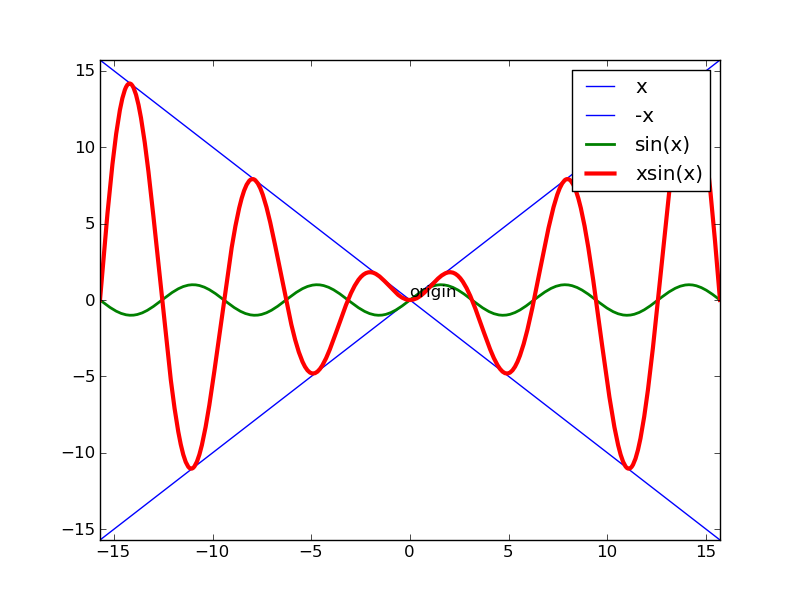
\includegraphics[scale=0.4]{four_plot}    
    \end{center}
\end{frame}
\begin{frame}[fragile]
\frametitle{Fix \texttt{linspace()} problem}
\label{sec-5}

\begin{verbatim}
   from scipy import *
\end{verbatim}
\end{frame}
\begin{frame}[fragile]
\frametitle{Fix \texttt{plot()} problem}
\label{sec-6}

\begin{verbatim}
   from pylab import *
\end{verbatim}
\end{frame}
\begin{frame}[fragile]
\frametitle{Better way of fixing}
\label{sec-7}

\begin{verbatim}
   from scipy import linspace
\end{verbatim}

  instead of
\begin{verbatim}
   from scipy import *
\end{verbatim}

    \texttt{*} means import all functions from name-space \texttt{scipy}.
\end{frame}
\begin{frame}[fragile]
\frametitle{Instead of \texttt{*}}
\label{sec-8}

\begin{verbatim}
    from scipy import linspace, pi, sin
    from pylab import plot, legend, annotate
    from pylab import xlim, ylim, title, show
\end{verbatim}

  Is better than, \texttt{from scipy import *} \& \texttt{from pylab import *}.
\end{frame}
\begin{frame}[fragile]
\frametitle{Another Fix}
\label{sec-9}

\begin{verbatim}
import scipy
import pylab
x = scipy.linspace(-5*scipy.pi, 5*scipy.pi, 500)
pylab.plot(x, x, 'b')
pylab.plot(x, -x, 'b')
pylab.plot(x, scipy.sin(x), 'g', linewidth=2)
pylab.plot(x, x*scipy.sin(x), 'r', linewidth=3)
pylab.legend(['x', '-x', 'sin(x)', 'xsin(x)'])
pylab.annotate('origin', xy = (0, 0))
pylab.xlim(-5*scipy.pi, 5*scipy.pi)
pylab.ylim(-5*scipy.pi, 5*scipy.pi)
\end{verbatim}
\end{frame}
\begin{frame}
\frametitle{Exercise 1}
\label{sec-10}

  Write a python script to plot a sine wave from 
    $-2\Pi$
  to 
    $2\Pi$
  .
\end{frame}
\begin{frame}
\frametitle{What is a module?}
\label{sec-11}

  Module is simply a file containing Python definitions and
  statements. Definitions from a module can be imported into other
  modules or into the main module.
\end{frame}
\begin{frame}
\frametitle{Python standard library}
\label{sec-12}

  Python has a very rich standard library of modules.
\begin{itemize}
\item Few libraries

\begin{itemize}
\item Math: \texttt{math}, \texttt{random}
\item Internet access: \texttt{urllib2}, \texttt{smtplib}
\item System, Command line arguments: \texttt{sys}
\item Operating system interface: \texttt{os}
\item regular expressions: \texttt{re}
\item compression: \texttt{gzip}, \texttt{zipfile}, \texttt{tarfile}
\end{itemize}

\item More information

\begin{itemize}
\item \href{http://docs.python.org/library}{http://docs.python.org/library}
\end{itemize}

\end{itemize}
\end{frame}
\begin{frame}
\frametitle{Summary}
\label{sec-13}

\begin{itemize}
\item Running scripts from command line
\item Learned about modules

\begin{itemize}
\item importing modules
\end{itemize}

\item Python standard library
\end{itemize}
\end{frame}
\begin{frame}
\frametitle{Thank you!}
\label{sec-14}

  \begin{block}{}
  \begin{center}
  This spoken tutorial has been produced by the
  \textcolor{blue}{FOSSEE} team, which is funded by the 
  \end{center}
  \begin{center}
    \textcolor{blue}{National Mission on Education through \\
      Information \& Communication Technology \\ 
      MHRD, Govt. of India}.
  \end{center}  
  \end{block}
\end{frame}

\end{document}
